\minitoc

% =============================================================================
% Généralités 

\section{Généralités}

\subsection{Un peu d'histoire...}

Nous sommes en été 1955 aux États-Unis. La naissance de l'informatique pousse les mathématiciens  John McCarthy, Marvin Minsky, Nathaniel Rochester et l'ingénieur Claude Shannon à proposer  un projet de recherche sur l'intelligence articielle au Dartmouth college "A proposal for the Dartmouth summer research project on artificial intelligence". Ils obtiennent ainsi 7500 \$ de la fonction Rockfeller  pour organiser un atelier de travail sur les machines pensantes durant deux mois. 
Cependant, l'intérêt pour ce domaine de recherche est encore très faible parmi la communauté scientifique.  Les faibles performances des premières machines constituent aussi un important frein au développement de prototypes. 

En 1957, Frank Rosenblatt présente le premier réseau de neurones tel que nous les connaissons aujourd'hui appelés \emph{Perceptron}. En 1986, la notion de Perceptron multicouches est explorée et en 1955 Yann LeCun et Yoshua Bengio
développe le premier réseau de neurones à convolution à la base de la vision par ordinateur. 

La victoire de DeepBlue sur Garry Kasparov aux échecs en 1997 démontre la puissance et le potentiel de ces  nouvelles technologies. L'affluence de données disponibles ces 30 dernières années et l'évolution  des capacités de calcul des ordinateurs a ouvert la porte à des systèmes de plus en plus performants.  Enfin, 2015 marque l'apogée des modèles d'IA dits "classiques" avec la victoire d'AlphaGo sur les champions  d'Europe et du monde. 

\subsection{Définition et terminologie}

Selon Wikipédia, l'intelligence artificielle se définit comme suit : 
\begin{quote}
    \emph{"L'intelligence artificielle (IA) est l'ensemble des systèmes informatiques capables d'effectuer des tâches  typiquement associées à l'intelligence, telles que l'apprentissage, le raisonnement, la résolution de problèmes, la perception ou la prise de décision."}
\end{quote}
Le but de l'IA est donc de reproduire numériquement le mode de pensée humaine. Ces concepts ont étés, et sont toujours,  à la base des réseaux de neurones actuels puisqu'ils sont contitués de neurones organisés en couches permettant de  traiter l'information. C'est donc une discipline très vaste dans lequel il est facile de confondre les notions. 

\medskip 

L'\emph{apprentissage automatique} en est un sous-domaine qui consiste en la création d'algorithmes capables  d'apprendre à partir de données précédement collectées.  Il faut donc distinguer plusieurs phases dans le processus de développement d'un tel modèle : 
\begin{enumerate}
    \item La collecte des données d'entraînement. 
    \item L'entraînement du modèle. 
    \item La phase de test des performances du modèle. 
    \item La mise sur le marché pour une utilisation publique. 
\end{enumerate}
Nous traiterons ici les phases 1 et 2 de ce processus. Les autres appartiennent à des domaines différents de l'IA.  Pour le développement d'un tel modèle, nous devons donc avoir accès à des \textbf{observations} consituées d'exemples ou de données collectés. Ces données sont consituées de deux éléments : les \textbf{attributs}, appelés \emph{features},  consituent des réprésentations numériques des observations et les \textbf{étiquettes}, ou \emph{labels}, qui  associent à chaque élément une catégorie ou une valeur. L'enjeu est donc d'entraîner un modèle à distinguer  les différents attributs pour chaque observation et d'être capable de répondre correctement à la question :  "Étant donné une observation, à quelle catégorie appartient-elle ?".  Pour cela, le jeu de données initial, appelée \emph{dataset}, sera séparé en deux, l'un pour l'entraînement, et l'autre  pour le test. 

\medskip

Plus formellement, pour un ensemble $E = \{(x_i, y_i) \mid i \in \llbracket 1, N \rrbracket\}$ de données consitué d'observation $X$ et de données $Y$, on 
cherche à apprendre une fonction $f$ telle que : 
    $$ f : 
        \begin{cases}
            X \longrightarrow Y \\ 
            x_i \longmapsto y_j = f(x_i)
        \end{cases}
    $$
et l'on souhaite que $i = j$ pour le plus de cas possibles. C'est-à-dire que notre modèle ne se trompe 
pas dans la prédiction $y_i$ de la classe de $x_i$. En fonction de la nature de l'ensemble $Y$, on distinguera plusieurs 
types de problèmes. Si $Y$ est un ensemble fini, on parlera de \emph{problème de classification}, si $Y = \{vrai, faux\}$, 
on parlera de \emph{prédiction} et si $Y = \R$, on parlera de régression. 

\subsection{L'apprentissage}

L'apprentissage constitue le cœur de ce que nous allons voir ici. Cette phase permet de définir "les bonnes réponses" 
au modèle. On distingue ainsi différents types d'apprentissages : 
\begin{itemize}
    \item \textbf{L'apprentissage supervisé} : on dispose ici de données étiquetées et le modèle 
    doit apprendre à distinguer les classes des observations. 
    \item \textbf{L'apprentissage non supervisé} : ici le modèle n'a accès qu'aux observations 
    et doit déterminer lui-même leur classes. 
    \item \textbf{L'apprentissage par renforcement} : le modèle est ici très différent, il se représente 
    sous la forme d'un agent devant apprendre une série d'actions en fonction de la configuration de son 
    environnement. Pour cela, à chaque essai, on lui attribue une récompense positive ou négative. 
\end{itemize}

Nous nous intéressons ici à l'apprentissage supervisé. 

% ========================================================================
% Perceptron et MLP 

\section{Du Perceptron au MLP}

Le \emph{Perceptron} peut être vu comme le premier réseau de neurones moderne, bien que sa conception date de 1956. À cette époque, Frank Rosenblatt pense à une "solution à tout" basée sur une représentation  simplifiée du cerveau humain. L'idée est de recréer un ensemble de neurones connectés les uns aux autres  capables d'"apprendre". 

\subsection{Concept}

On se pose donc un problème à deux classes $(c_-, c_+)$ avec $m$ exemples : 
    $$ \mathcal{D} = \{(x_i, y_i) \in \R^p \times \{-1, 1\} \mid j \in \llbracket 1,m \rrbracket\} $$
Pour chaque exemple, $x_i$ représente l'observation et $y_i$ la classe correspondante. On veut  développer un modèle capable de déterminer la classe d'une observation brute.  On effectue donc une hypothèse forte qui est que les deux classes $c_-$ et $c_+$ sont séparables  par un hyperplan de $ \R^p$. Le problème revient donc à construire une famille $(w_1, \dots, w_p)$  de \emph{poids} qui définiront cet hyperplan. Formellement, on veut "apprendre" une fonction $y$ telle que : 
    $$ \forall i \in \llbracket 1, m \rrbracket, \quad 
        y(x) = 
            \begin{cases}
                1 \text{ si } \sum_{j=1}^{p} w_j x_j > T \\
                -1 \text{ sinon} 
            \end{cases}.
    $$
On appellera cette fonction $y$, notée $ \hat{y}$ la \emph{prédiction}. Ici notre réseau de neurones a déjà  pris forme. Il se représente encore plutôt sous la forme d'un neurone : 
    
    \begin{figure}[H]
        \centering
        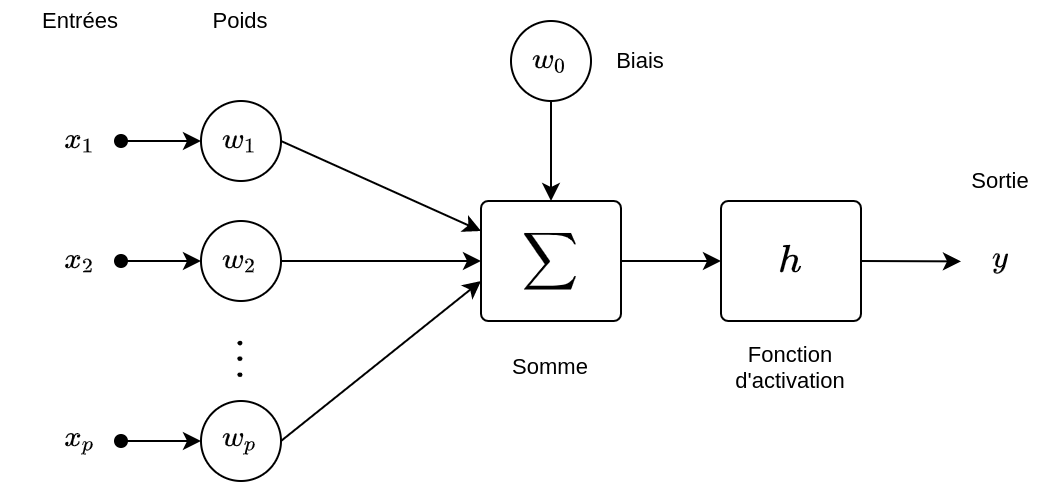
\includegraphics[scale=0.3]{./images/neurone_formel.png}
        \label{img:neurone}
        \caption{Schéma formel d'un neurone}
    \end{figure}

On utilisera aussi une \emph{fonction d'activation} représentée par le seuil $T$. Plus tard, nous utiliserons  des fonctions plus complexes pour donner une valeur de "probabilité" à la sortie d'un neurone. 

\subsection{Apprentissage}

Une fois la structure posée, nous devons définir un algorithme pour apprendre les poids  $(w_1, \dots, w_p)$ dans le but d'avoir une séparation optimale des deux classes dans $\R^p$.  L'idée est donc de faire passer des valeurs $x$ dans le perceptron et d'actualiser les poids  $w_j$ si la prédiction $ \hat{y}$ est différente de la classe $y$.  Une règle simple d'actualisation est de modifier $w_j$ en fonction de la valeur $x_j$ de l'entrée  qu'il pondère. On aura donc la règle suivante : 
    $$ 
        w = 
        \begin{cases}
            w + x \text{ si } y = 1 \text{ et } \hat{y} = -1 \\
            w - x \text{ si } y = - 1 \text{ et } \hat{y} = 1
        \end{cases}
        \quad \iff \quad 
        w = w + y x \text{ si } x \text{ est mal classé}.
    $$

\begin{remark}[Variantes]
    Notre définition de l'actualisation des poids les modifie à chaque itération lors de l'apprentissage. Cela permet une convergence rapide de l'apprentissage, mais peut conduire à une instabilité  si le nombre de poids à traiter est trop grand.  Une solution est donc d'effectuer un \emph{apprentissage par batch}. Cela consiste à faire  passer successivement plusieurs vecteurs $x$, on calcule ensuite l'erreur moyenne commise et on met à jour les poids en fonction de cette erreur moyenne. 
    Un autre possibilité est d'utiliser un \emph{learning rate} $ \nu$ qui bride l'apprentissage. On utilise alors la règle suivante pour actualier $w$ : 
        $$ w = \eta  (y - \hat{y}) x. $$
\end{remark}

Les perceptrons permettent donc de simuler des fonctions booléennes comme illustré ci-dessous : 

% Style mis à jour
\tikzset{
    int/.style={draw, circle, fill=gray!20, minimum size=2.5em, thick},
    input/.style={draw, circle, fill=white!10, minimum size=2em}
}

\begin{figure}[h!]
    \centering
    \begin{minipage}{0.45\textwidth}
        \centering
        \begin{tikzpicture}[auto, >=Stealth, node distance=1.5cm, scale=0.8, transform shape]
        
            % --- NOEUDS ---
            % Le neurone central
            \node [int] (a) {$\Sigma$};

            % Entrées x1 et x2 (positionnées par rapport à 'a')
            \node [input] (x2) [left=1.5cm of a] {$x_2$};
            \node [input] (x1) [above=0.5cm of x2] {$x_1$};
            \node [input] (x3) [below=0.5cm of x2] {$1$};

            % Le Biais arrivant par le haut
            \node (bias_in) [above=1.2cm of a] {$0$};

            % --- FLÈCHES ET POIDS ---
            % Entrées vers neurone avec poids sur les flèches
            \path[->, thick] (x1) edge node[above] {$-1$} (a);
            \path[->, thick] (x2) edge node[above] {$-1$} (a);
            \path[->, thick] (x3) edge node[below] {$-1.5$} (a);
            
            % Flèche du biais
            \path[->, thick] (bias_in) edge (a);

            % Sortie vers la formule
            \node (output) [right=1.0cm of a] {};
            \path[->, thick] (a) edge (output);

            % --- FORMULE À DROITE ---
            \node[right=0cm of output, font=\Large] (formula) {
                $y = x_1 \land x_2$
            };

            % Optionnel : annotation sous la formule pour expliquer la fonction
            % \node[below=0.1cm of formula, font=\small\itshape, text width=4cm, align=center] {
            %     Simule la fonction porte \\ \textbf{NON-ET (NAND)}
            % };
        \end{tikzpicture}
        \captionof{figure}{Fonction AND avec un perceptron}
    \end{minipage}
    \hfill
    \begin{minipage}{0.45\textwidth}
        \centering
        \begin{tikzpicture}[auto, >=Stealth, node distance=1.5cm, scale=0.8, transform shape]
        
            % --- NOEUDS ---
            % Le neurone central
            \node [int] (a) {$\Sigma$};

            % Entrées x1 et x2 (positionnées par rapport à 'a')
            \node [input] (x2) [left=1.5cm of a] {$x_2$};
            \node [input] (x1) [above=0.5cm of x2] {$x_1$};
            \node [input] (x3) [below=0.5cm of x2] {$1$};

            % Le Biais arrivant par le haut
            \node (bias_in) [above=1.2cm of a] {$0$};

            % --- FLÈCHES ET POIDS ---
            % Entrées vers neurone avec poids sur les flèches
            \path[->, thick] (x1) edge node[above] {$-1$} (a);
            \path[->, thick] (x2) edge node[above] {$-1$} (a);
            \path[->, thick] (x3) edge node[below] {$-0.5$} (a);
            
            % Flèche du biais
            \path[->, thick] (bias_in) edge (a);

            % Sortie vers la formule
            \node (output) [right=1.0cm of a] {};
            \path[->, thick] (a) edge (output);

            % --- FORMULE À DROITE ---
            \node[right=0cm of output, font=\Large] (formula) {
                $y = x_1 \lor x_2$
            };

            % Optionnel : annotation sous la formule pour expliquer la fonction
            % \node[below=0.1cm of formula, font=\small\itshape, text width=4cm, align=center] {
            %     Simule la fonction porte \\ \textbf{NON-ET (NAND)}
            % };
        \end{tikzpicture}        
        \captionof{figure}{Fonction OR avec un perceptron}
    \end{minipage}
\end{figure}

Après réflexion, on se rend compte qu'il est impossible de simuler la fonction XOR  avec un seul neurone. Ce sera donc l'objectif des \emph{MLP (Multi Layer Perceptron)}  composés de plusieurs couches de neurones interconnectés. 


\subsection{Perceptron Multi-Couches (MLP)}

Comme énoncé précédemment, le perceptron simple de Rosenblatt présente une limitation fondamentale mise en lumière par Marvin Minsky et Seymour Papert en 1969 : l'impossibilité géométrique de séparer des classes qui ne sont pas linéairement séparables dans l'espace d'entrée $\R^d$, à l'instar de la fonction logique $\mathrm{XOR}$ (ou exclusif).

Pour contourner ce problème, l'approche naturelle consiste à empiler plusieurs couches de neurones formels. Un \emph{Perceptron Multi-Couches} (Multi-Layer Perceptron, noté MLP) est composé :
\begin{enumerate}
    \item D'une couche d'entrée (vecteur $x \in \R^d$) ;
    \item D'une suite de $L \geqslant 1$ \textbf{couches cachées} (hidden layers), qui apprennent des représentations hiérarchiques distribuées ;
    \item D'une couche de sortie produisant la prédiction $\hat{y}$.
\end{enumerate}

\begin{definition}[Formalisation de la passe avant d'un MLP]
    Soit un réseau à $L$ couches cachées. Notons $h^{(0)} = x \in \R^{d_0}$ le vecteur d'entrée. Pour chaque couche $k \in \llbracket 1, L \rrbracket$ de dimension $d_k$, le vecteur d'activation est régi par les relations de récurrence :
    \begin{align}
        a^{(k)} &= W^{(k)} h^{(k-1)} + b^{(k)} \in \R^{d_k} \quad &\text{(pré-activation)} \\
        h^{(k)} &= g^{(k)}\left(a^{(k)}\right) \in \R^{d_k} \quad &\text{(activation)}
    \end{align}
    où $W^{(k)} \in \R^{d_k \times d_{k-1}}$ désigne la matrice de poids de la couche $k$, $b^{(k)} \in \R^{d_k}$ le vecteur de biais associé, et $g^{(k)} : \R \to \R$ une fonction d'activation non linéaire appliquée composante par composante.
    Pour la couche de sortie $k = L+1$, on applique une fonction terminale $o$ :
    \begin{equation}
        \hat{y} = h^{(L+1)} = o\left(W^{(L+1)} h^{(L)} + b^{(L+1)}\right).
    \end{equation}
\end{definition}

\begin{remark}[Interprétation géométrique des frontières de décision]
    Chaque neurone d'une première couche cachée partitionne l'espace $\R^d$ par un demi-espace délimité par un hyperplan affine. Les neurones de la deuxième couche cachée effectuent une intersection booléenne (opérateur $\mathrm{ET}$) de ces demi-espaces, formant ainsi des polyèdres convexes. Enfin, les couches suivantes peuvent réaliser l'union (opérateur $\mathrm{OU}$) de régions convexes disjointes, rendant le réseau théoriquement capable d'approximer n'importe quelle frontière de décision fermée ou ouverte arbitrairement complexe.
\end{remark}

% =============================================================================
% Fonctions d'activation et Classification linéaire multiclasse

\section{Fonctions d'Activation et Classification Multiclasse}

\subsection{Fonctions d'activation usuelles}

Le choix d'une fonction d'activation non linéaire $g$ est indispensable : sans elle, la composition successive d'opérations affines $W^{(L)}(\dots (W^{(1)}x + b^{(1)}) \dots) + b^{(L)}$ resterait strictement équivalente à une unique transformation affine globale $\tilde{W}x + \tilde{b}$, ruinant tout l'intérêt de la profondeur.

\begin{definition}[Fonctions d'activation courantes]
    On définit ainsi différentes fonctions d'activations communément utilisées en sortie d'un neuronne. Pour tout réel $z \in \R$ on a :
    \begin{itemize}
        \item \textbf{Sigmoïde (logistique)} : 
        \begin{equation}
            \sigma(z) = \frac{1}{1 + e^{-z}}. 
        \end{equation}
        Elle projette $\R$ sur $]0, 1[$ et vérifie l'identité remarquable $\sigma'(z) = \sigma(z)(1 - \sigma(z))$.
        \item \textbf{Tangente hyperbolique} : 
        \begin{equation}
            \tanh(z) = \frac{e^z - e^{-z}}{e^z + e^{-z}} \in ]-1, 1[, 
        \end{equation}
        centrée en zéro, de dérivée $\tanh'(z) = 1 - \tanh^2(z)$.
        \item \textbf{Rectified Linear Unit (ReLU)} : 
        \begin{equation}
            g(z) = \max(0, z).
        \end{equation}
        Sa dérivée vaut $1$ pour $z > 0$ et $0$ pour $z < 0$. Elle évite la saturation des gradients pour des entrées positives.
        \item \textbf{Leaky ReLU} : pour $\alpha \in ]0, 1[$ (couramment $\alpha = 0{,}01$), $g(z) = \max(\alpha z, z)$. Elle évite le problème des "neurones morts" lorsque $z < 0$.
        \item \textbf{Softplus} : 
        \begin{equation}
            g(z) = \log(1 + e^z),
        \end{equation}
        approximation analytique différentiable de la ReLU.
    \end{itemize}
\end{definition}

\subsection{Classification multiclasse et fonction Softmax}

Considérons un problème de classification à $K > 2$ classes mutuellement exclusives. La couche finale produit un vecteur de scores réels non normalisés $a = W^{(L+1)}h^{(L)} + b^{(L+1)} \in \R^K$, appelés \emph{logits}.

\begin{definition}[Opérateur Softmax]
    L'opérateur Softmax normalise un vecteur de logits $a = (a_1, \dots, a_K)^\top$ en une distribution discrète de probabilités $p = (p_1, \dots, p_K)^\top \in [0, 1]^K$ définie par :
    \begin{equation}
        \forall c \in \llbracket 1, K \rrbracket, \quad p_c = \operatorname{Softmax}(a)_c = \frac{e^{a_c}}{\sum_{j=1}^{K} e^{a_j}}.
    \end{equation}
    On a immédiatement $\forall c, \; p_c > 0$ et $\sum_{c=1}^K p_c = 1$. La classe prédite est $\hat{y} = \arg\max_{c} p_c$.
\end{definition}

% =============================================================================
% Fonctions de perte

\section{Fonctions de Perte (\emph{Loss Functions})}

En apprentissage supervisé, puisque nous connaissons les \emph{labels} associés à chaque prédiction, nous sommes capables d'évaluer le modèle en temps réel sur chacune de ses prédiction sur les données d'entraînement. Ainsi, l'évaluation de la discordance entre la cible réelle $y$ et la sortie estimée $\hat{y}$ s'effectue au moyen d'une fonction de coût différentiable $\mathcal{L}(y, \hat{y})$ que l'on appellera \emph{fonction de perte} ou \emph{loss}. 

\subsection{Entropie croisée binaire (BCE)}

\begin{remark}[Limites de la MSE]
    Pour une classification binaire avec $y \in \{0, 1\}$ et une prédiction de probabilité $\hat{y} = \sigma(z) \in ]0, 1[$, l'erreur quadratique usuelle MSE s'avère sous-optimale du fait de zones de saturation où le gradient s'annule pour des erreurs maximales. On introduit la perte d'entropie croisée binaire.    
\end{remark}

\begin{definition}[Binary Cross-Entropy]
    Pour $y \in \{0, 1\}$ et $\hat{y} \in ]0, 1[$ :
    \begin{equation}
        \mathcal{L}_{\mathrm{BCE}}(y, \hat{y}) = - y \log(\hat{y}) - (1 - y) \log(1 - \hat{y}).
    \end{equation}
\end{definition}

\begin{proposition}[Stabilité numérique de la BCE]
    En injectant l'activation logistique $\hat{y} = \sigma(z) = \frac{1}{1 + e^{-z}}$ directement dans la perte, on évite les dépassements de capacité flottante (\emph{overflow}) via l'expression analytique exacte :
    \begin{equation}
        \mathcal{L}_{\mathrm{BCE}}(y, \sigma(z)) = \max(z, 0) - z \cdot y + \log\left(1 + e^{-|z|}\right).
    \end{equation}
\end{proposition}

% TODO : Ajouter d'autres fonctions de perte


% =============================================================================
% Rétropropagation et Dérivation Automatique

\section{Rétropropagation du Gradient et Dérivation Automatique}

Comme vu au début de ce chapitre, l'apprentissage se fait par une recherche des "meilleurs" poids possibles pour le modèle dans l'objectif de minimiser l'erreur commise. Maintenant que nous avons introduit la fonciton de perte \emph{loss}, nous cherchons donc à faire une minimisation de cette fonction \emph{loss}. 

La principale problématique dans ce processus est le calcul de son \emph{gradient}. En effet, pour trouver des candidats minimiseurs, la condition d'optimalité d'ordre 1 nous demande d'annuler ce gradient. Nous devons donc être capable de calculer les dérivées partielles de la \emph{loss} en fonction des poids du modèle. On utilise pour cela l'algorithme de \emph{rétropropagation} à l'aide de \emph{graphes computationnels}. 

\subsection{Rétropropagation sur un neurone formel}

Considérons un unique neurone formel doté d'une entrée $x \in \R^d$, d'une pré-activation $a = w^\top x + b$, d'une activation $\hat{y} = \sigma(a)$, et d'une perte quadratique $\mathcal{L} = \frac{1}{2}(y - \hat{y})^2$. Par application directe de la règle de dérivation en chaîne (\emph{Chain Rule}) :
\begin{equation}
    \frac{\partial \mathcal{L}}{\partial w_i} = \frac{\partial \mathcal{L}}{\partial \hat{y}} \cdot \frac{d\hat{y}}{da} \cdot \frac{\partial a}{\partial w_i} = - (y - \hat{y}) \cdot \hat{y}(1 - \hat{y}) \cdot x_i.
\end{equation}
On retrouve le terme d'erreur $(y - \hat{y})$, pondéré par la pente de la sigmoïde $\hat{y}(1 - \hat{y})$ et la projection d'entrée $x_i$. Si l'on remplace la perte quadratique par la $\mathcal{L}_{\mathrm{BCE}}$, le terme $\hat{y}(1-\hat{y})$ se simplifie élégamment au dénominateur :
\begin{equation}
    \frac{\partial \mathcal{L}_{\mathrm{BCE}}}{\partial a} = \hat{y} - y \implies \frac{\partial \mathcal{L}_{\mathrm{BCE}}}{\partial w} = (\hat{y} - y)x.
\end{equation}

\subsection{Rétropropagation dans un MLP (\emph{Backpropagation})}

% TODO : Rajouter partie graphe computationnel et exemple de calcul à la main

Dans un graphe multicouches, les erreurs locales sont propagées de l'aval vers l'amont :
\begin{definition}[Rétropropagation multicouche]
    Posons $\delta^{(k)} = \frac{\partial \mathcal{L}}{\partial a^{(k)}}$ le vecteur de sensibilité de la couche $k$.
    \begin{align}
        \text{Couche de sortie } (L+1) : \quad \delta^{(L+1)} &= \nabla_{a^{(L+1)}} \mathcal{L} \\
        \text{Couches cachées } (k = L, \dots, 1) : \quad \delta^{(k)} &= \left( (W^{(k+1)})^\top \delta^{(k+1)} \right) \odot g'^{(k)}\left(a^{(k)}\right)
    \end{align}
    où $\odot$ désigne le produit d'Hadamard (terme à terme). Les gradients s'en déduisent immédiatement :
    \begin{equation}
        \frac{\partial \mathcal{L}}{\partial W^{(k)}} = \delta^{(k)} \left(h^{(k-1)}\right)^\top \in \R^{d_k \times d_{k-1}}, \qquad \frac{\partial \mathcal{L}}{\partial b^{(k)}} = \delta^{(k)} \in \R^{d_k}.
    \end{equation}
\end{definition}

\subsection{Graphes de calcul et implémentation PyTorch}

En pratique, le calcul symbolique manuel des dérivées est remplacé par l'auto-différenciation en mode inverse (\emph{reverse-mode automatic differentiation}) matérialisée par un graphe acyclique orienté (DAG). 

\begin{lstlisting}[language=Python, caption={Implémentation d'un MLP complet sous PyTorch}]
import torch
import torch.nn as nn

class MultiLayerPerceptron(nn.Module):
    def __init__(self, in_features: int, hidden_dim: int, out_classes: int):
        super(MultiLayerPerceptron, self).__init__()
        self.network = nn.Sequential(
            nn.Linear(in_features, hidden_dim),
            nn.ReLU(),
            nn.Linear(hidden_dim, hidden_dim),
            nn.ReLU(),
            nn.Linear(hidden_dim, out_classes)
        )
        
    def forward(self, x: torch.Tensor) -> torch.Tensor:
        # Retourne les logits bruts (non normalises)
        return self.network(x)

# Instanciation et passe avant/arriere
model = MultiLayerPerceptron(in_features=784, hidden_dim=128, out_classes=10)
criterion = nn.CrossEntropyLoss() # Integre log-softmax et NLL
optimizer = torch.optim.SGD(model.parameters(), lr=0.01, momentum=0.9)

x_dummy = torch.randn(32, 784) # Batch de 32 observations
y_target = torch.randint(0, 10, (32,))

optimizer.zero_grad()
logits = model(x_dummy)
loss = criterion(logits, y_target)
loss.backward() # Calcul automatique des gradients via Autograd
optimizer.step()
\end{lstlisting}

\subsection{Optimisation par descente de gradient avec inertie (Momentum)}

La descente de gradient stochastique standard (SGD) présente de fortes oscillations transverses dans les vallées mal conditionnées (matrice hessienne à fort conditionnement). La méthode avec moment régularise la trajectoire en accumulant une moyenne exponentielle glissante des vitesses passées :
\begin{align}
    v_t &= \beta v_{t-1} + \alpha \nabla_W \mathcal{L}_t \quad \text{avec } \beta \in [0, 1[ \\
    W_{t+1} &= W_t - v_t
\end{align}
où $\alpha > 0$ représente le pas d'apprentissage (\emph{learning rate}).

% TODO : Rajouter autres params et optimiseurs